%\documentclass[preprint,12pt,times]{elsarticle}

%% Use the option review to obtain double line spacing
%% \documentclass[preprint,review,12pt]{elsarticle}

%% Use the options 1p,twocolumn; 3p; 3p,twocolumn; 5p; or 5p,twocolumn
%% for a journal layout:
%% \documentclass[final,1p,times]{elsarticle}
%% \documentclass[final,1p,times,twocolumn]{elsarticle}
%% \documentclass[final,3p,times]{elsarticle}
%% \documentclass[final,3p,times,twocolumn]{elsarticle}
%% \documentclass[final,5p,times]{elsarticle}
 \documentclass[final,5p,times,twocolumn]{elsarticle}

%% if you use PostScript figures in your article
%% use the graphics package for simple commands
%% \usepackage{graphics}
%% or use the graphicx package for more complicated commands
%% \usepackage{graphicx}
%% or use the epsfig package if you prefer to use the old commands
%% \usepackage{epsfig}

%% The amssymb package provides various useful mathematical symbols
\usepackage{amssymb}
%% The amsthm package provides extended theorem environments
%% \usepackage{amsthm}

%% The lineno packages adds line numbers. Start line numbering with
%% \begin{linenumbers}, end it with \end{linenumbers}. Or switch it on
%% for the whole article with \linenumbers after \end{frontmatter}.
\usepackage{lineno}

\biboptions{sort&compress}

\usepackage{amsmath}
\usepackage{textcomp} %Permet d'introduire un mu droit à l'aide de \textmu en dehors de l'environnement math
\usepackage{color}

\usepackage[leftbars]{changebar} %Pour insérer une barre de mise à  jour (à  gauche car [leftbars]) au moyen de \begin{changebar} %Ne fonctionne pas pour passer du DVI au pdf -> utiliser DV -> PS -> pdf

\usepackage{multirow}
%\usepackage{rotating} %Pour effectuer la rotation d'un tableau à  l'aide de "\begin{sidewaystable} et \end{}" et supprimer "\begin{table} et \end{}"
\usepackage{pdflscape}
\usepackage{tikz}
\usetikzlibrary{patterns}
\usepackage{pgfplots}

%\newcommand{\e}[1]{\exp\left({#1}\right)}
\newcommand{\e}[1]{\mbox{\ensuremath{\mathrm{e}^{#1}}}}
\DeclareMathOperator{\sigmoid}{sig}

\journal{CIRP Journal of Manufacturing Science and Technology}

\begin{document}

%%%%%%%%%%%%%%%%%%%%%%%%%%
\begin{frontmatter}

\title{Predictive 3D modelling of free oblique cutting of Ti6Al4V titanium alloy and experimental validation for a wide range of conditions}

\author[1]{F. Ducobu\corref{cor1}}
\ead{Francois.Ducobu@umons.ac.be}
\cortext[cor1]{Corresponding author. Tel.: +32 65 45 68}

\author[2]{O. Pantal\'{e}}
\author[1]{E. Rivi\`{e}re-Lorph\`{e}vre}
\author[3]{B. Lauwers}

\address[1]{Machine Design and Production Engineering Lab, Research Institute for Science and Material Engineering, UMONS, Belgium}
\address[2]{Laboratoire G\'{e}nie de Production, INP/ENIT, Universit\'{e} de Toulouse, Tarbes, France}
\address[3]{Department of Mechanical Engineering, KU Leuven \& Flanders Make@KU Leuven-MaPS, Belgium}

%%%%%%%%%%%%%%%%%%%%%%%%%%
\begin{abstract}

Modelling of the cutting process needs to move from a 2D to a 3D configuration to get closer to industrial applications. The study introduces a predictive 3D finite element model of free orthogonal and oblique cutting with an ANN-based material constitutive model and experimental validation in strictly the same conditions (cutting and geometrical). Predictive performance of the model is high for the forces in the 3 directions and the chip thickness ratio on all 36 cutting conditions (including 2 inclination angles). Accuracy of the main cutting force is excellent: the mean difference with the experiments is 3\%.

\end{abstract}
%%%%%%%%%%%%%%%%%%%%%%%%%%

%%%%%%%%%%%%%%%%%%%%%%%%%%
\begin{keyword}
%% keywords here, in the form: keyword \sep keyword

Oblique cutting \sep Finite element method (FEM) \sep Predictive model \sep Artificial Neural Network (ANN)

\end{keyword}
%%%%%%%%%%%%%%%%%%%%%%%%%%

\end{frontmatter}
%%%%%%%%%%%%%%%%%%%%%%%%%%

%%
%% Start line numbering here if you want
%%
\linenumbers

%% main text
%%%%%%%%%%%%%%%%%%%%%%%%%%
\section{Introduction}
\label{Intro}
%%%%%%%%%%%%%%%%%%%%%%%%%%

Selection of the tools and the cutting conditions in machining, but also comprehension of the influence of the process parameters on the quality of a component and its optimisation, are still difficult to achieve because of the high level of complexity and linked nonlinear involved phenomena. In the frame of digital manufacturing and Industry 4.0, modelling of the cutting process supports them, while remaining a challenging task. As highlighted by Arrazola et al. \cite{arrazola_recent_2013}, most finite element (FE) models are developed in 2D (orthogonal cutting configuration usually) although industrial applications require a 3D modelling.

The experimental configuration to validate a model must be as close as possible to the simulation. Few configurations in strictly orthogonal cutting conditions are found. Broaching \cite{abouridouane_friction_2021} or milling \cite{sela_measurement_2021, ducobu_experimental_2015} machines are mostly used; dedicated machines such as in \cite{afrasiabi_numerical-experimental_2021} allow for high cutting speed. Free oblique cutting with a straight cutting edge has not been studied yet: all the efforts have been focussing on orthogonal cutting (mostly for 2D validation).

Lagrangian and Eulerian formulations are the most used for FE modelling of the cutting process. The Coupled Eulerian-Lagrangian (CEL) formulation has recently been successfully applied to the modelling of cutting (2D orthogonal configuration): it provides accurate results with a realistic chip shape and no mesh distortion \cite{ducobu_application_2016}. First applications in 3D are found in recent works \cite{xu_simulation_2021, ducobu_finite_2017, ambrosio_new_2022, vovk_finite_2020, hardt_three_2021}. They mostly cover (free) orthogonal cutting, while free oblique cutting still needs to be investigated.

The behaviour of the machined material is one of the key aspects of a FE model \cite{arrazola_recent_2013, melkote_advances_2017}. Research is very intense in this field, which leads to a growing number of material constitutive models ranging from empirical to physical models \cite{melkote_advances_2017}. The empirical Johnson-Cook (JC) model \cite{johnson_constitutive_1983} is still the most used so far. One issue of material behaviour modelling for cutting simulation is the identification of the model parameters, moreover as the experimental equipment does not allow to reach the high levels of strains, strain rates and temperature of machining \cite{melkote_advances_2017}. Inverse identification is an alternative, but the uniqueness of the solution is not always guaranteed \cite{arrazola_recent_2013}. It uses optimisation or Artificial Intelligence based methods \cite{melkote_advances_2017}, such as in \cite{hardt_investigations_2021}, and requires defining the analytical expression of the constitutive model.

This paper fills the literature gap on oblique cutting by investigating free orthogonal and oblique 3D cutting configurations from both the experimental and the numerical points of view. An Artificial Neural Network (ANN), introduced in \cite{pantale_efficient_2022}, is implemented in a FE cutting model for the first time instead of the analytical JC law. A broad range of cutting speeds (6), uncut chip thicknesses (3) and inclination angles (2) resulting in 36 different conditions are considered to demonstrate the predictive ability of the FE model for fundamental variables. No assumptions are made about the geometry of the machined workpiece in the model (i.e. its width is the same as in the experiments), while keeping computation time relevant for industrial applications. The developments apply to the titanium alloy Ti6Al4V.

%%%%%%%%%%%%%%%%%%%%%%%%%%
\section{Experimental setup}
\label{ExpSet}
%%%%%%%%%%%%%%%%%%%%%%%%%%

A 3-axis GF Mikron VCE 600 Pro milling machine is used to carry out dry free orthogonal and oblique cutting tests on Ti6Al4V (grade 5 annealed at 750°C for 1 h followed by air cooling) with the same kinematics as a shaper. As shown in Figure \ref{ExpSetup}, the tungsten carbide tool (modified LCGN160602-0600-FG, CP500 from SECO) is fixed on a dedicated holder (modified CFHN-06 from SECO) and the sample to be cut is clamped in the spindle (no rotation is allowed during the test). The top of the sample includes 3 ribs of 1 mm in width (width of the tool is 6 mm) and 10 mm in length. The test consists of removing the upper layer (its height is the uncut chip thickness, $h$) of one rib at the prescribed cutting speed, $v_c$. The cutting speed is provided by the feed rate, $v_f$, of the machine (max. value of 40 m/min). The tool cutting edge inclination, $\lambda_s$, results from the orientation of the tool and the sample. Forces are measured with a 3-component Kistler 9257B dynamometer and are amplified by a Kistler 5070A charge amplifier. Acquisition is performed at 3 kHz with a Kistler 5697A2 data acquisition system and the DynoWare software. Table \ref{tab:CutCond} shows the cutting conditions, each is repeated 3 times.

\begin{figure}[h]
\centering
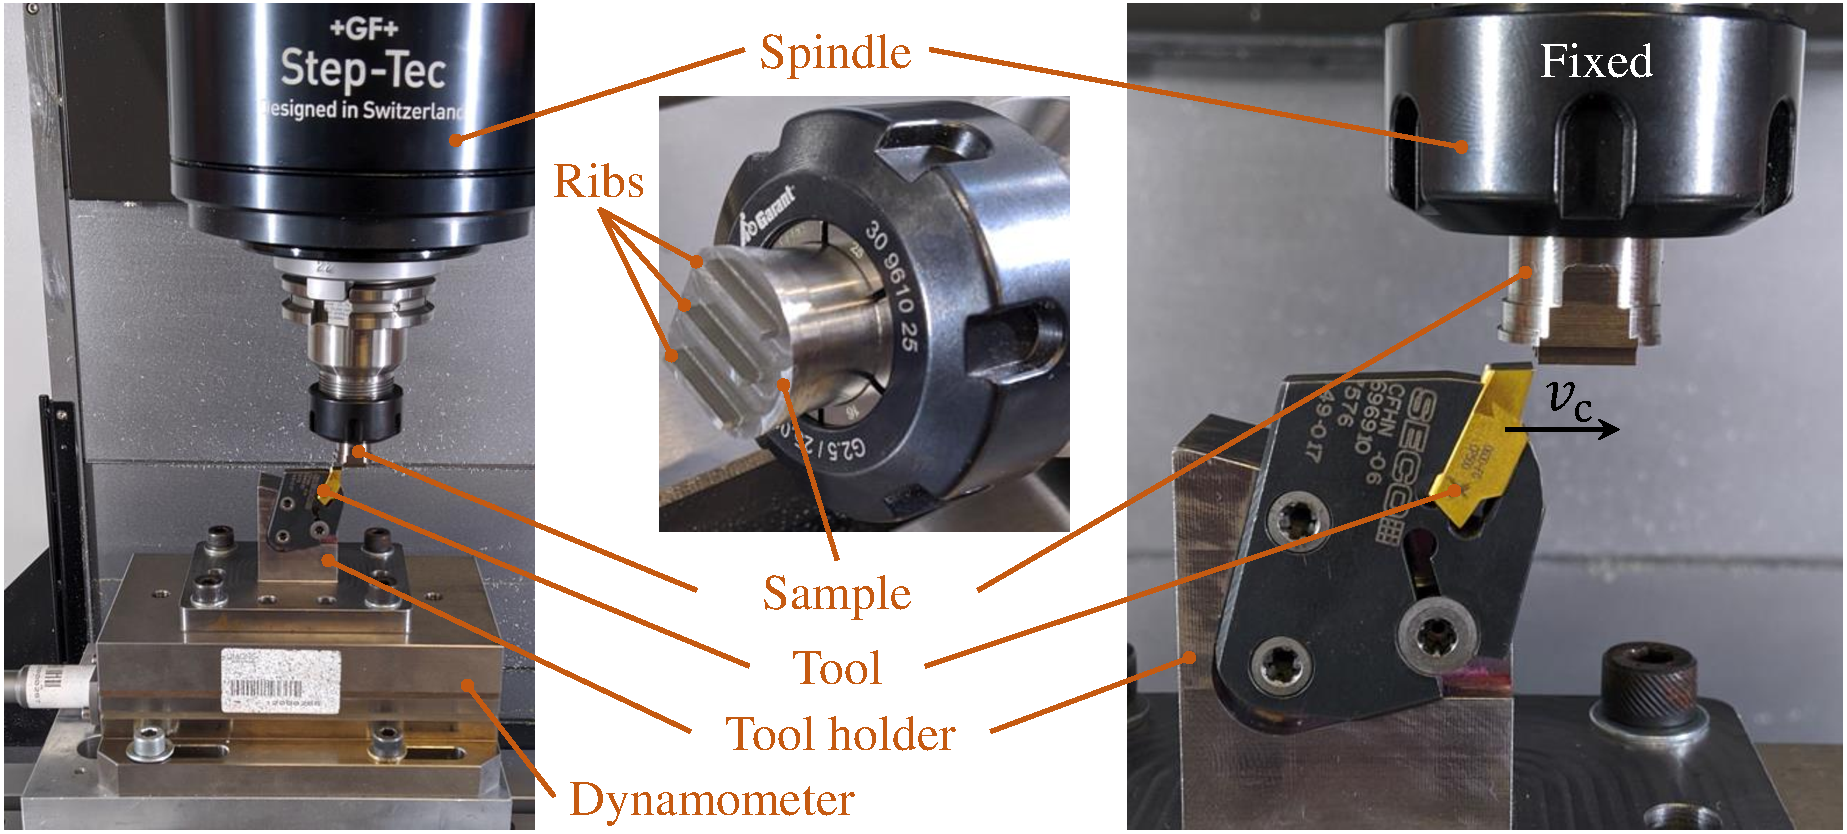
\includegraphics[width=\columnwidth]{Figures/ExpSetup}
\caption{Experimental setup}
\label{ExpSetup}
\end{figure}

%
\begin{table}[!h]
\begin{center}
\caption{\label{tab:CutCond} Cutting conditions of the study}
\begin{tabular}{ll}
\hline\noalign{\smallskip}
Parameter  & Values\\
\noalign{\smallskip}\hline\noalign{\smallskip}
Cutting speed, $v_c$ (m/min) & 5, 7.5, 10, 20, 30, 40\\
Uncut chip thickness, $h$ (\textmu{}m) & 40, 60, 80\\
Cutting edge inclination, $\lambda_s$ & 0, 6\\
Width of the workpiece (mm) & 1\\
Length of the workpiece (mm) & 10\\
Width of the cutting edge (mm) & 6 (1.1 in the model)\\
Cutting edge radius, $r_\beta$ (\textmu{}m) & 20\\
Rake angle, $\gamma_0$ (\textdegree{}) & 15\\
Clearance angle, $\alpha_0$ (\textdegree{}) & 2\\
\noalign{\smallskip}\hline
\end{tabular}
\end{center}
\end{table}
%

%%%%%%%%%%%%%%%%%%%%%%%%%%
\section{Finite element model}
\label{FEM}
%%%%%%%%%%%%%%%%%%%%%%%%%%

\subsection{Modelling choices}

The CEL formulation is adopted to model the dry free orthogonal and oblique cutting tests with Abaqus/Explicit 2020. The 3D model is composed of a fixed Lagrangian tool and a Eulerian workpiece (Figure \ref{BC}). Chip formation occurs by plastic flow across the Eulerian domain with no mesh distortion. The Eulerian formulation enables to form chips without damage properties, removing modelling assumptions. These two characteristics contribute to cutting models providing accurate results and realistic chips \cite{ducobu_application_2016}.

\begin{figure}[h]
\centering
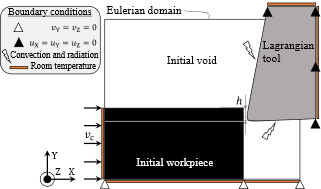
\includegraphics[width=\columnwidth]{Figures/BC}
\caption{Boundary conditions and schematic initial geometry of the model}
\label{BC}
\end{figure}

As shown in Figure \ref{FEConfig}, the full width of the workpiece (1 mm) is modelled. To allow chip formation and side flow, the Eulerian domain is wider (it includes the volume in which material can move). The volume above the initial workpiece is also meshed with Eulerian elements for the same reasons. As in the experiments and to fulfil the hypothesis of free orthogonal and oblique cutting, the tool is wider than the workpiece (it is of 1.1 mm in the model and of 6 mm in the experiments). It is very important to stress that the models are the same for both inclination angles: they only differ by the rotation of the tool of 6° about Y axis as in the experiments (Figure \ref{FEConfig}). This, coupled to the absence of assumptions when developing the models, contributes to make the models predictive.

\begin{figure}[h]
\centering
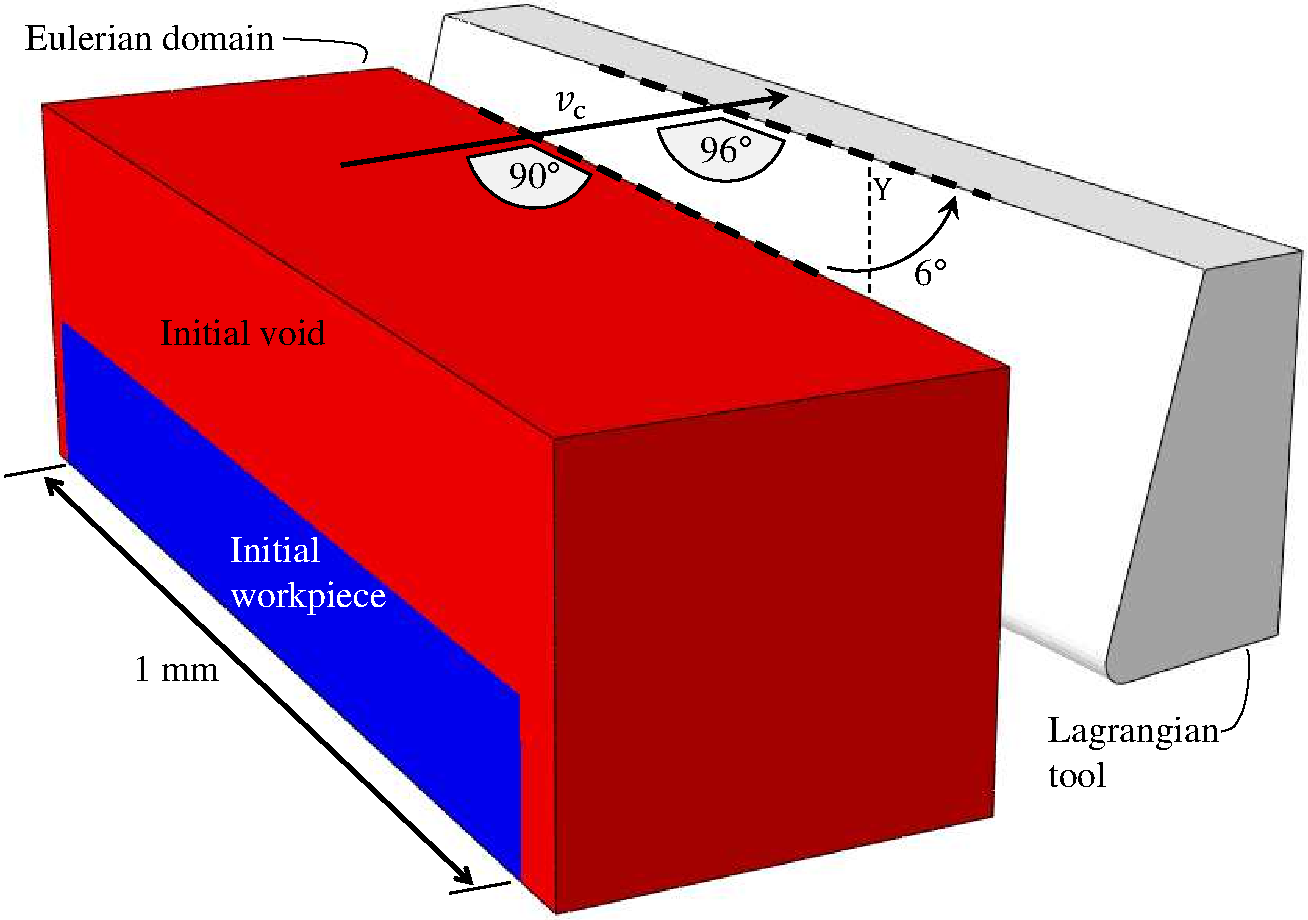
\includegraphics[width=\columnwidth]{Figures/FEConfig}
\caption{Configuration of the FE model for $\lambda_s$ = 6°}
\label{FEConfig}
\end{figure}

According to a previous mesh sensitivity study in orthogonal cutting with CEL \cite{ducobu_finite_2017}, elements edge size is 5 µm in the plane parallel to the cutting speed. In the direction perpendicular to this plane, it is 5 µm in areas close to the lateral boundaries of the Eulerian domain and 50 µm in the middle of the workpiece. To reduce computation time, the size of the model depends on the value of the uncut chip thickness. This results in a Eulerian domain (EC3D8RT linear 3D Eulerian elements with 8 nodes, coupled mechanical-thermal behaviour and reduced integration) composed of 216,550 to 273,350 nodes and a Langrangian domain (C3D8T linear 3D Lagrangian elements with 8 nodes, coupled mechanical-thermal behaviour and reduced integration) of 4,650 nodes.

The Ti6Al4V workpiece is assumed to be thermo-elasto-viscoplastic (isotropic) and inelastic heat fraction is 0.9. The tungsten carbide tool with TiN coating is assumed to be linear elastic. Material properties are provided in Table \ref{tab:prop}.

%
\begin{table}[!h]
\begin{center}
\caption{\label{tab:prop} Materials properties \cite{Seo2004, Granta, Milosevic}}
\begin{tabular}{lll}
\hline\noalign{\smallskip}
Young's modulus, $E$ (GPa) & Ti6Al4V & 113.8$^*$\\
 & WC & 650\\
Poisson's ratio, $\nu$ & Ti6Al4V & 0.34\\
 & WC & 0.2\\
Density, $\rho$ (kg/m$^3$) & Ti6Al4V & 4,430\\
 & WC & 14,850\\
Conductivity, $k$ (W/mK) & Ti6Al4V & 6.3$^*$\\
 & WC & 100\\
Expansion, $\alpha$ (K$^{-1}$) & Ti6Al4V & 8.6 e$^{-6*}$\\
 & WC & 5 e$^{-6}$\\
Specific heat, $c_{p}$ (J/KgK) & Ti6Al4V & 531$^*$\\
 & WC & 202\\
\noalign{\smallskip}\hline\noalign{\smallskip}
JC constitutive model & $A$ (MPa) & 997.9\\
 & $B$ (MPa) & 653.1\\
 & $C$ & 0.0198\\
 & $m$ & 0.7\\
 & $n$ & 0.45\\
 & $\dot{\varepsilon}_{0}$ (s$^{-1}$) & 1\\
 & $T_{\text{room}}$ (K) & 293\\
 & $T_{\text{melt}}$ (K) & 1873\\
\noalign{\smallskip}\hline\noalign{\smallskip}
\end{tabular}
\end{center}
\vspace{-0.4cm}$^*$: Dependence to the temperature, value provided at 293 K
\end{table}
%

Following the experimental results of Rech et al. \cite{rech_characterisation_2013}, Coulomb's friction is assumed to occur at the tool-workpiece interface and both friction and heat partition coefficients depend on the cutting speed. Limiting shear stress is included + equa. All the friction energy is converted into heat. Table XX shows the friction parameters adopted in this study.

%
Table friction
%

Room temperature of 293 K is imposed on the upper and right surfaces of the tool and on the left and bottom surfaces of the workpiece (Figure 2). Radiation and convection are assumed to occur on the rake and clearance faces of the tool. Initial temperature of the tool and the workpiece is set to room temperature (293 K).

\subsection{Material constitutive model of Ti6Al4V}

The constitutive model of the Ti6Al4V material used in all the numerical simulations proposed in section \ref{sec:ExpNumResults} is a thermo-elasto-viscoplastic law using a flow criterion based on an artificial neural network (ANN) identified for the selected material and implemented in the Abaqus/Explicit code via a Fortran routine VUHARD as proposed by Pantalé et al. in \cite{pantale_efficient_2022}.
The principle of this approach consists in replacing the analytical formulation of the flow law, based on a Johnson-Cook or Zerilli-Armstrong type model, and allowing the calculation of the flow stress $\sigma^y$ as a function of the plastic strain $\varepsilon^p$, of the plastic strain rate, ${\dot{\varepsilon}}^p$, and of the temperature $T$, by a multi-layer ANN serving as universal approximator. Thus, we can directly identify the parameters of the neural network from the experimental data without having to postulate a behavioural model, which simplifies the procedure and allows more flexibility in the definition of the model.
The proposed approach also allows, as shown in Pantalé et al. \cite{pantale_efficient_2022}, to compute the derivatives of the flow stress $\sigma^y$ with respect to the three input variables of the model, a necessary step to implement this model as a flow law in the form of a VUHARD subroutine in the Abaqus/Explicit FEM code.

In order to verify the influence of the complexity of the neural network on the numerical results of the simulation and the computing time, several architectures of ANN are tested thereafter. The chosen global architecture has 2 hidden layers with a variable number of neurons for the first hidden layer ($\zeta$ = 9 to 17) and 7 neurons for the second hidden layer, 3 inputs (plastic strain, $\varepsilon^p$, plastic strain rate, ${\dot{\varepsilon}}^p$, and temperature, T) and one output (the yield stress, $\sigma^y$). The global architecture of this kind of ANN is given in Figure \ref{ANN}.

\begin{figure}[h]
\centering
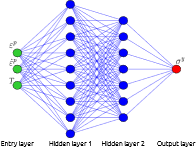
\includegraphics[width=0.8\columnwidth]{Figures/ANN}
\caption{Architecture of the ANN 3-9-7-1-sig used for the flow law}
\label{ANN}
\end{figure}

A Sigmoid activation function defined by equation (\ref{eq:sigmoid}) is used for all neurons in the two hidden layers, but none is used for the output neuron.
\begin{equation}
\sigmoid(x)=\frac{1}{1 + \e{-x}}\label{eq:sigmoid}
\end{equation}
Because of the large number of identified parameters for the whole ANN model (from 122 to 210 for 9 and 17 neurons for the first hidden layer, respectively); the 5 sets of ANN parameters used in this publication are provided in \cite{pantale_coefficients_2022}.

\subsection{Sensitivity study of the results to mass scaling}

FE modelling of the cutting process is very expensive in CPU computation time because of the coupling on many nonlinear phenomena and the large amount of tiny finite elements. Mass scaling (MS) is introduced in the model to reduce the CPU computation time while checking that it does not influence the results (forces and energies) via a mass scaling sensitivity study.
MS factors, ${MS}_f$, ranging from 1E6 (theoretical scaling of CPU time of 1000) to 1 (no scaling) have been used for one cutting condition ($\lambda_s$ = 0°, $v_c$ = 30 m/min and h = 60 µm). Table \ref{tab:MS} gives the results normalised ($\hat{x}$) by these of the model without MS (x). As expected, actual speed-up does not increase linearly with the ${MS}_f$, but it is still significant. ${MS}_f$ of 1E6 leads to unstable computation and ${MS}_f$ of 1E5 results in erratic forces evolutions. These results are confirmed by high values of the kinetic ($KE$) on internal ($IE$) energies ratio (it should not exceed a few \%). A ${MS}_f$ value of 1E3 is selected as it provides a good balance between computation time reduction and impact on forces (considered in the analysis), while keeping $\frac{KE}{IE}$ below 1\%. To provide an order of magnitude of CPU computation time, between 10 h and 50 h are needed on 4 cores of an Intel i7-5700 HQ at 3.48 GHz.

%
\begin{table}[!h]
\begin{center}
\caption{\label{tab:MS} MS sensitivity study (selected $MS_f$ in bold)}
\begin{tabular}{lllll}
\hline\noalign{\smallskip}
$MS_f$  & Speed-up & $\hat{F_c}$ & $\hat{F_f}$ & $\frac{KE}{IE}$ (\%)\\
\noalign{\smallskip}\hline\noalign{\smallskip}
1 & 1 & 1 & 1 & 2.3E-4\\
1E2 & 9 & 1.006 & 0.982 & 2.2E-2\\
\textbf{1E3} & \textbf{21} & \textbf{1.008} & \textbf{0.940} & \textbf{2.2E-1}\\
1E4 & 61 & 1.012 & 0.921 & 2.4\\
1E5 & 173 & Erratic & Erratic & 22\\
1E6 & 207 & Unstable & Unstable & 58\\
\noalign{\smallskip}\hline
\end{tabular}
\end{center}
\end{table}
%

\subsection{Sensitivity study of the results to the number of neurons}

The number of neurons on the hidden layers may influence the results. A sensitivity study on the number of neurons for the first hidden layer is carried out to select the ANN providing the best balance between CPU computation time and quality of the results. The study shows no influence on the forces when compared to the built-in Johnson-Cook model, only computation time is influenced (Table \ref{tab:NbNeurons}). A first hidden layer with 9 neurons is therefore selected.

%
\begin{table}[!h]
\begin{center}
\caption{\label{tab:NbNeurons} Sensitivity to the number of neurons of the first layer, $\zeta$
(selection in bold)}
\begin{tabular}{llll}
\hline\noalign{\smallskip}
$\zeta$  & Time increase (\%) & $\hat{F_c}$ & $\hat{F_f}$\\
\noalign{\smallskip}\hline\noalign{\smallskip}
Built-in & 0 & 1.000 & 1.000\\
\textbf{9} & \textbf{6} & \textbf{1.000} & \textbf{0.999}\\
11 & 6 & 1.001 & 1.000\\
13 & 7 & 1.000 & 0.998\\
15 & 8 & 1.001 & 1.001\\
17 & 10 & 1.000 & 1.000\\
\noalign{\smallskip}\hline
\end{tabular}
\end{center}
\end{table}
%

%%%%%%%%%%%%%%%%%%%%%%%%%%
\section{Experimental and numerical results\label{sec:ExpNumResults}}
\label{Results}
%%%%%%%%%%%%%%%%%%%%%%%%%%

Experimental and numerical forces are filtered with a second-order low-pass Bessel filter at 750 Hz before computing the mean value of the signal at steady state. Mean and standard deviation ($2\sigma$) are computed from the 3 experimental values and are shown in Figures 5 to 7. Mean numerical values are plotted inside the experimental bars in Figures 5 to 7.

\begin{figure}[h]
\centering
\includegraphics[width=\columnwidth]{Figures/ExpNum_Forces_v10_40µ_6}
\caption{Temporal evolutions of experimental (E) and numerical (N) forces at 6°, 10 m/min and 40 \textmu{}m: dispersion around mean experimental values and linear extrapolation of numerical values in dashed}
\label{ExpNum_Forces_v10_40µ_6}
\end{figure}

\begin{figure}[h]
\centering
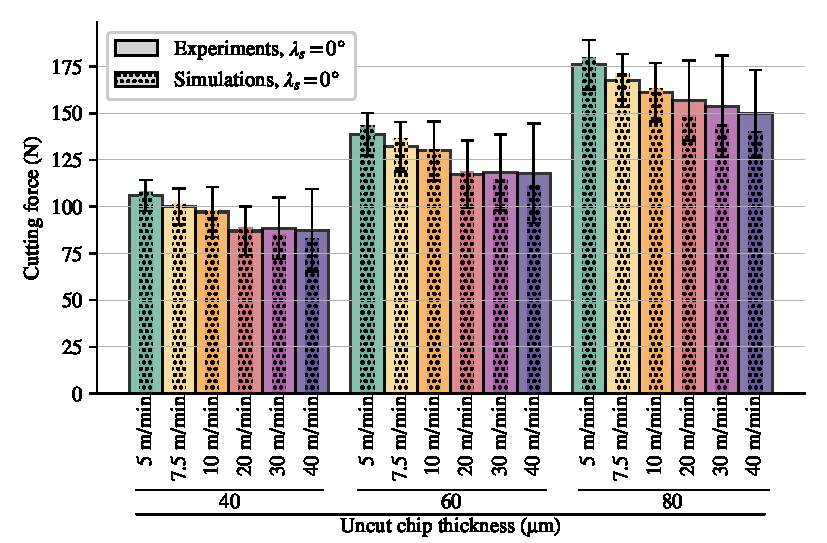
\includegraphics[width=\columnwidth]{Figures/Fx_0}
\caption{Comparison of experimental (E) and numerical (N) cutting forces at 0°}
\label{Fx_0}
\end{figure}

\begin{figure}[h]
\centering
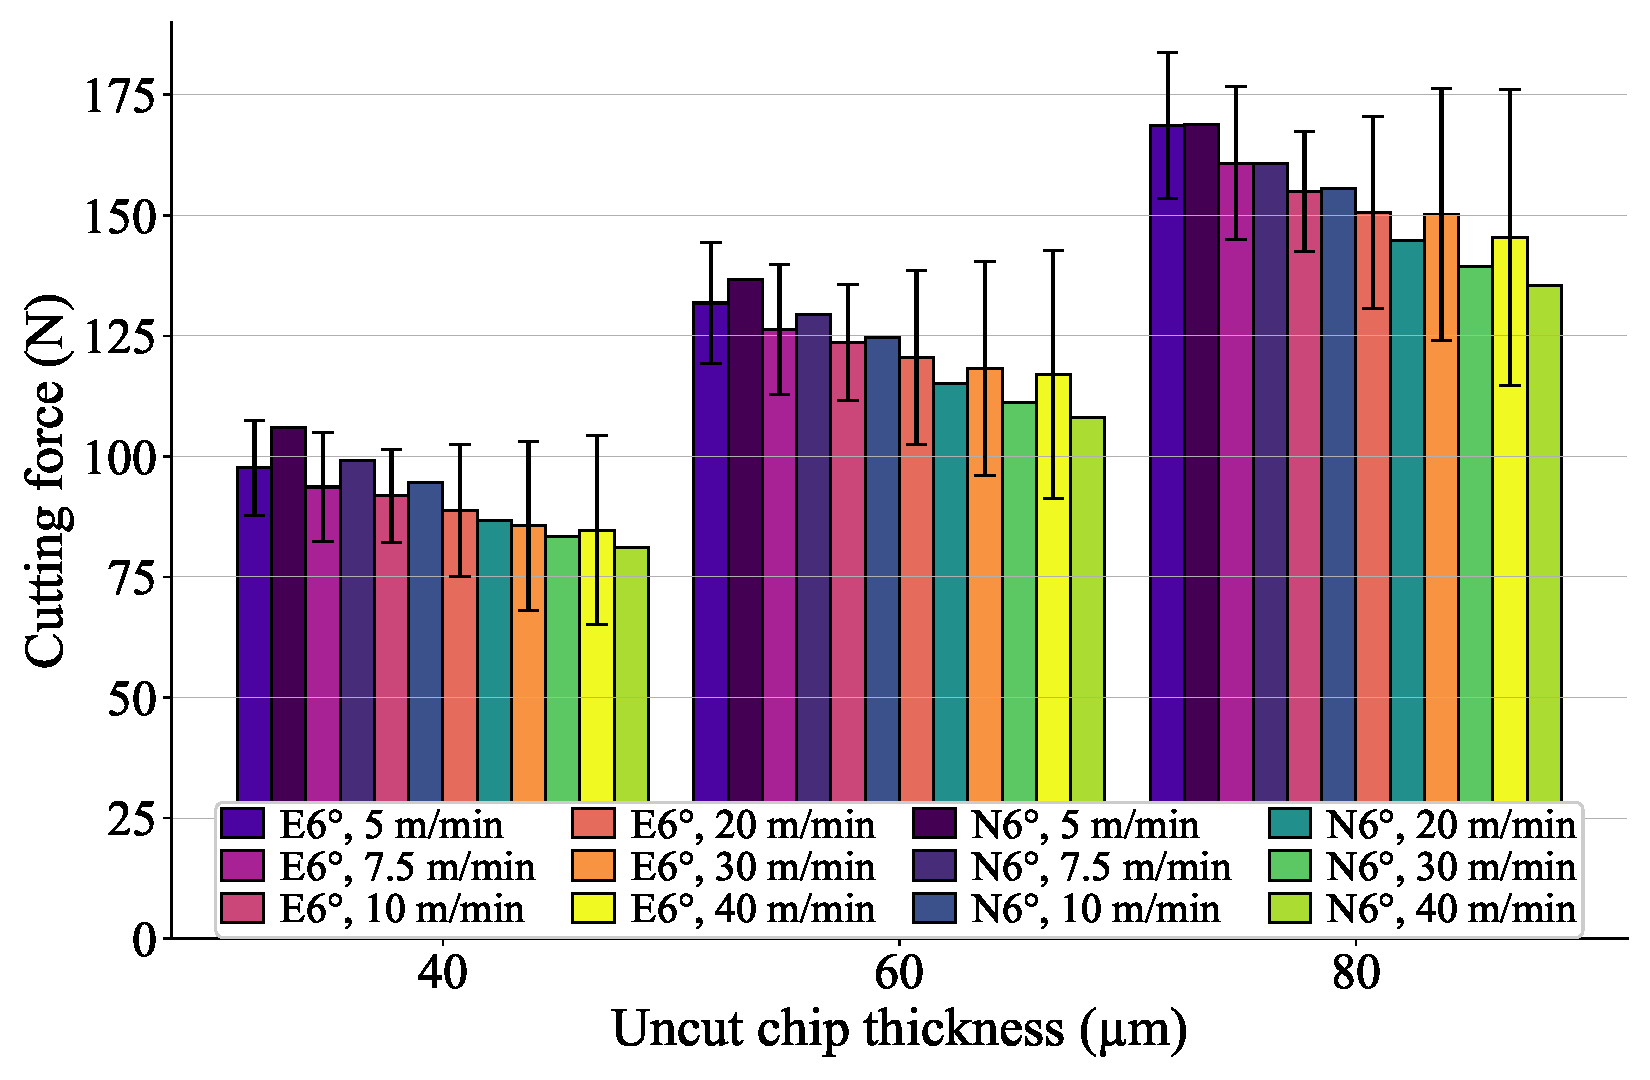
\includegraphics[width=\columnwidth]{Figures/Fx_6}
\caption{Comparison of experimental (E) and numerical (N) cutting forces at 6°}
\label{Fx_6}
\end{figure}

\begin{figure}[h]
\centering
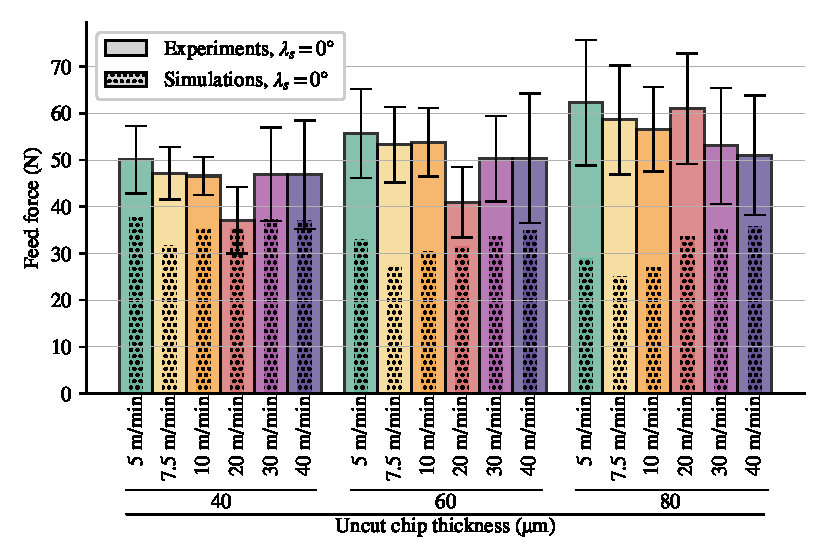
\includegraphics[width=\columnwidth]{Figures/Fy_0}
\caption{Comparison of experimental (E) and numerical (N) feed forces at 0°}
\label{Fy_0}
\end{figure}

\begin{figure}[h]
\centering
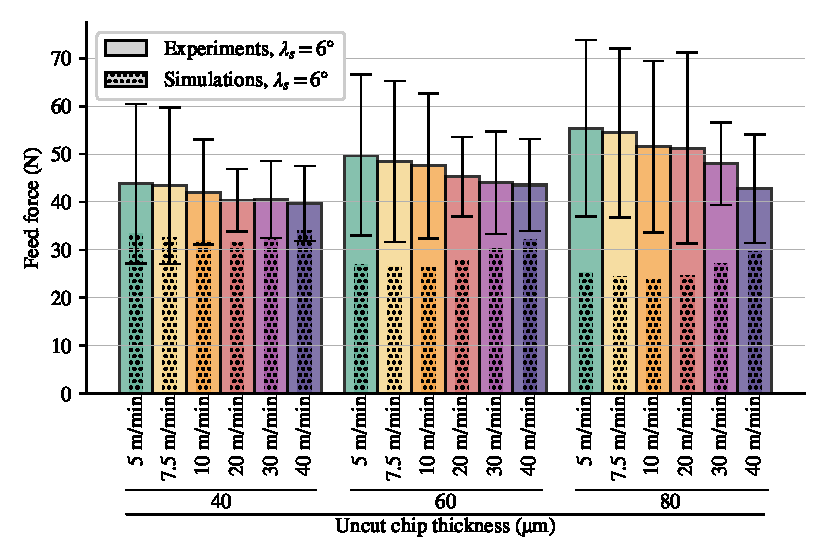
\includegraphics[width=\columnwidth]{Figures/Fy_6}
\caption{Comparison of experimental (E) and numerical (N) feed forces at 6°}
\label{Fy_6}
\end{figure}

\begin{figure}[h]
\centering
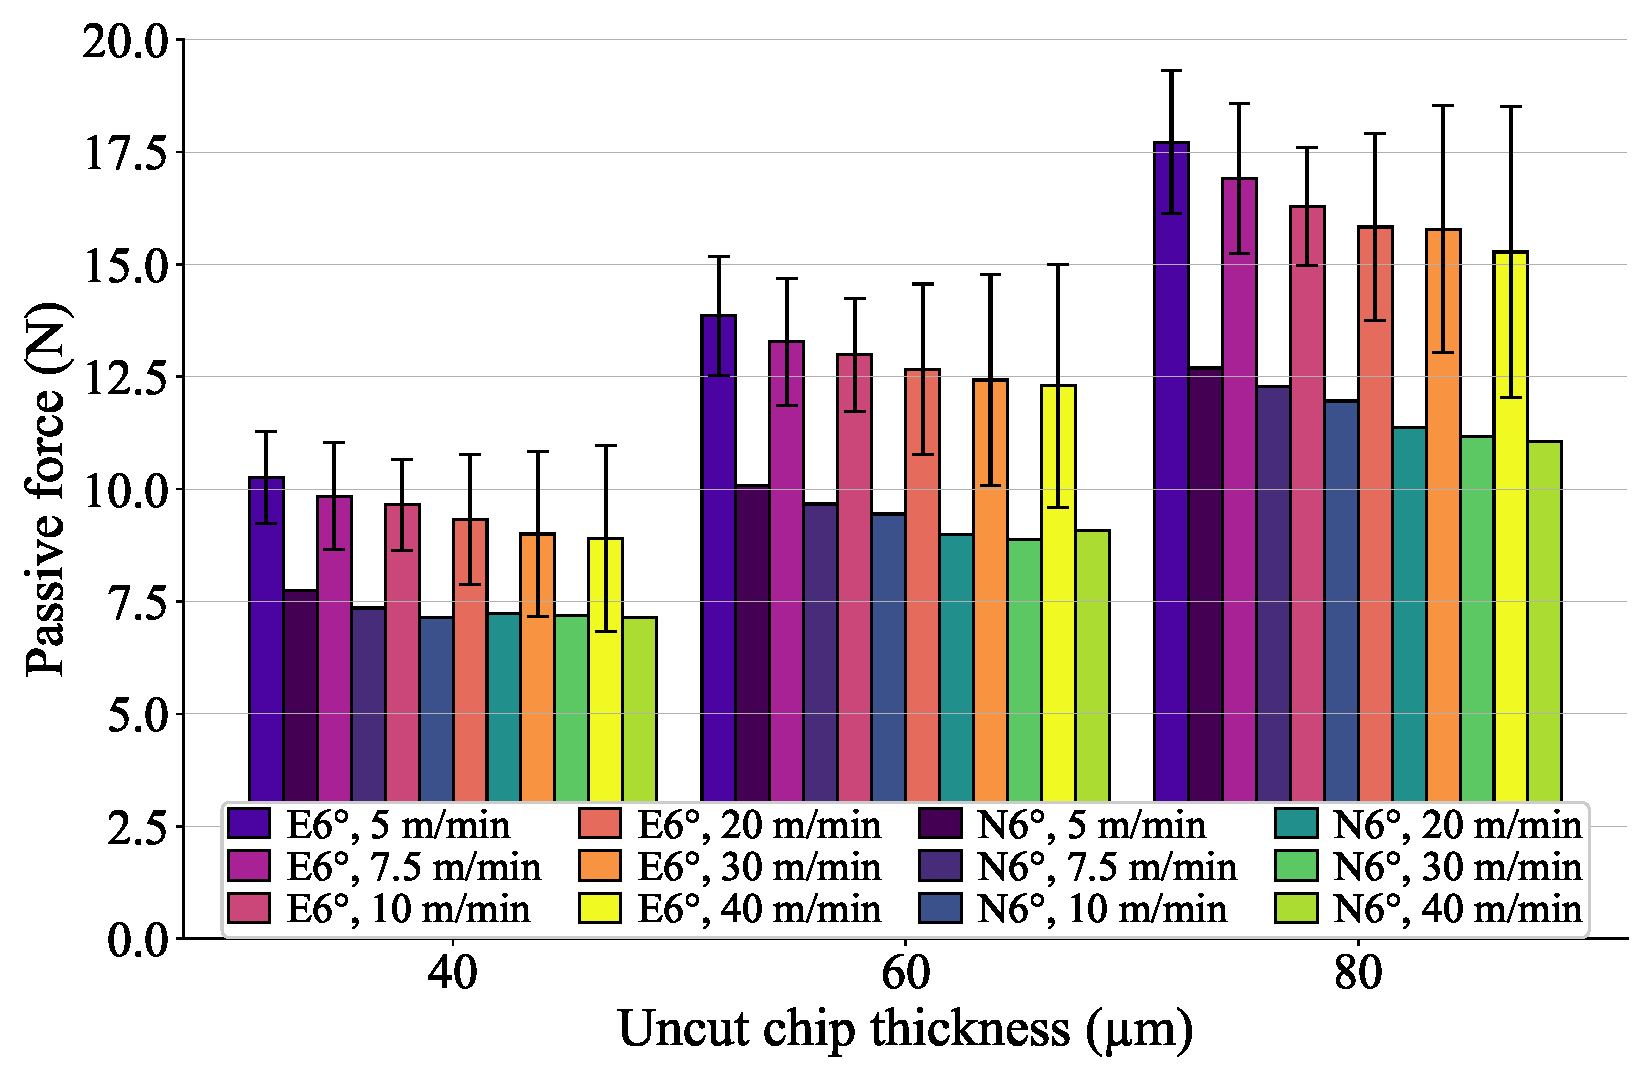
\includegraphics[width=\columnwidth]{Figures/Fz_6}
\caption{Comparison of experimental (E) and numerical (N) passive forces at 6°}
\label{Fz_6}
\end{figure}

The increase of the cutting force with the uncut chip thickness is clearly observed in Figure 5 for both experimental and numerical results at the 2 inclination angles, as well as the decrease of the force with the increase in the cutting speed. This shows temperature softening domination on strain rate hardening for Ti6Al4V and that it is accurately modelled. The increase of the inclination angle from 0° to 6° reduces the cutting force; this is well captured by the model. For cutting speeds of 20-40 m/min, $F_c$ is almost constant for 40 µm and 60 µm, while it slightly decreases for 80 µm; this small stabilisation is less marked for the model.
Increase in the deviation around the mean value with the cutting speed is noted for values above 10 m/min. All numerical values are within a confidence interval of 95\% of the experiments (35 out of 36 conditions are within a confidence interval of 68\%) and the mean difference with the experiments is 3\%, which is remarkable, moreover given the wide range of cutting conditions considered. This highlights the predictive qualities of the FE model for both inclination angles.
Figure 6 shows the results for the feed force, where the two clearest trends are its decrease with inclination angle and its increase with the uncut chip thickness for both experimental and numerical results. For 80 µm, $F_f$ globally decreases with $v_c$ in the experiments. For 40 and 60 µm, the force decreases at lower $v_c$ and then increases for 0°, while a decrease is observed at all $v_c$ for 6°. For the numerical values, the global trend is the same for the 3 uncut chip thicknesses and both inclination angles: a decrease for the lowest $v_c$ values and then an increase. The numerical values are mostly not within the 95\% confidence interval (it has no clear evolution with the cutting conditions). Coupled with the differences in trends, it shows that $F_f$ is less well modelled (mean difference is 35\%) as usual in FE modelling of the cutting process. Improving the friction model should enhance the results.
Passive force is non-zero for the inclination angle of 6° (Figure 7). As the cutting force, it increases with the uncut chip thickness and it decreases with the cutting speed. Comparison with the experiments is globally the same as for $F_c$, except for a larger difference in the magnitude of $F_p$ (mean difference is 26\%, but it is small in absolute – less than 5 N). The numerical values are mostly not in the 95\% experimental confidence interval.
Regarding the chips morphology, all of them are continuous. For both the simulation and the experiments, the chip thickness ratio, $\lambda_h$, decreases with the cutting speed because of reduction of friction and it is almost independent of the uncut chip thickness. The mean difference between experimental and numerical $\lambda_h$ is 13\% across the whole range of cutting conditions.

%%%%%%%%%%%%%%%%%%%%%%%%%%
\section{Conclusions}
%%%%%%%%%%%%%%%%%%%%%%%%%%

In this paper, an experimental study has been carried out in free orthogonal and oblique cutting for Ti6Al4V. It is a reference to assess the performances of the 3D FE model introducing an ANN-based constitutive model and developed in the same conditions. An unpreviously seen wide range of cutting conditions, 36, is considered, including 2 inclination angles.
Accurate evaluation of fundamental variables in 3D with the absence of tuning of both numerical parameters and model features when cutting conditions and inclination angle are significantly modified is a strong novelty of this work. Only changing the inclination angle to move from free orthogonal to oblique cutting while maintaining the quality of the results has no equivalent in the current literature, moreover as no study on free oblique cutting is available. Predictive abilities of the model make it adequate for development of tools with a straight cutting edge, for example.

%%%%%%%%%%%%%%%%%%%%%%%%%%%
%%% The Appendices part is started with the command \appendix;
%%% appendix sections are then done as normal sections
%%% \appendix
%
%%% \section{}
%%% \label{}
%
%%% References
%%%
%%% Following citation commands can be used in the body text:
%%% Usage of \cite is as follows:
%%%   \cite{key}          ==>>  [#]
%%%   \cite[chap. 2]{key} ==>>  [#, chap. 2]
%%%   \citet{key}         ==>>  Author [#]
%
%%% References with bibTeX database:
%
\bibliographystyle{model1-num-names}
\bibliography{Biblio}
%
%%% Authors are advised to submit their bibtex database files. They are
%%% requested to list a bibtex style file in the manuscript if they do
%%% not want to use model1-num-names.bst.
%
%%% References without bibTeX database:
%
%% \begin{thebibliography}{00}
%


%%% \bibitem must have the following form:
%%%   \bibitem{key}...
%%%
%
%% \bibitem{}
%
%% \end{thebibliography}
%

\end{document}
